\chapter{Grundlagen}
\label{cha:Fundamentals}

\section{AR.Drone 2.0}
%Christoph
Bei der AR.Drone 2.0 handelt es sich um einen ferngesteuerten Quadrocopter des französischem Herstellers Parrot SA. \cite{drone} Die Drohne ist standardmäßig steuerbar mit einer mobilen Applikation für Android und iOS Geräte. Dafür baut sie ein WLAN Netzwerk auf, mit dem sich die Geräte verbinden können. Zur Steuerung stellt die AR.Drone ein Interface zur Verfügung, mit dem sie ferngesteuert werden kann. \newline
Im Umfang der Studienarbeit wird, wie in der folgenden Abbildung zu sehen, die aktuellste Version der AR.Drone 2.0 verwendet. \newline
\begin{figure}[ht]
	\centering
	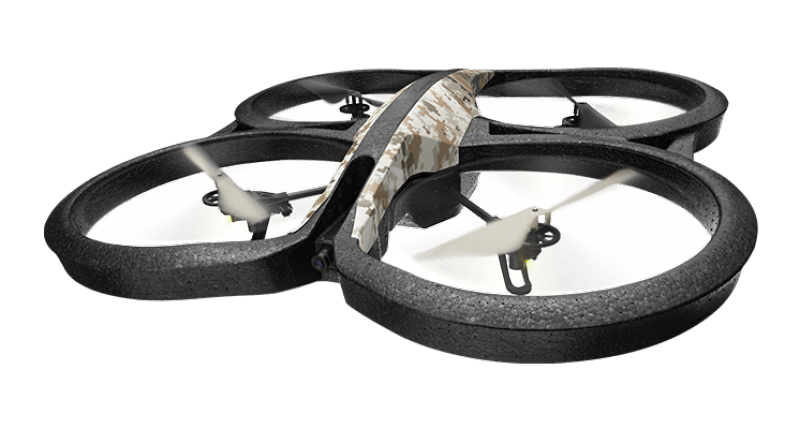
\includegraphics[scale=0.5]{Bilder/ar_drone.png}
	\caption{Parrot AR.DRONE 2.0 Elite Edition \cite{dronepicture}}
	\label{fig:ardrone}
\end{figure}

%https://www.parrot.com/fr/sites/default/files/styles/product_teaser_hightlight/public/parrot_ar_drone_gps_edition.png?itok=0shlzcXW
Diese zeichnet sich unter Anderem durch eine Frontkamera mit einer Auflösung von 1280×720 Pixeln und einer Bildrate von 30 fps aus. Weiterhin ist Sie mit einer zum Boden gerichteten QVGA Kamera ausgerüstet, welche 60 Bilder pro Sekunde aufnimmt. \newline
Die Drohne orientiert sich beim Fliegen mit Hilfe einer Vielzahl von Sensoren. Dazu gehören ein dreiachsiges Gyroskop und ein Magnetometer. Weiterhin nutzt sie Beschleunigungs-, Ultraschall- und Luftdrucksensoren. \newline
Der Grund für die Wahl der Drohne ist vor allem der vergleichsweise niedrige Preis von ca. 200€ und der starken Verbreitung in der Forschung. Dadurch gibt es bereits eine Vielzahl von Projekten, die dazu führen, dass die Drohne und das dazugehörige Interface zu einem großen Umfang fehlerfrei funktionieren. \newline
Weiterhin gibt es schon ROS Nodes (siehe \ref{ROS}) und konfigurierte Modelle in Simulationsumgebungen, welche die Arbeit an dem Projekt beschleunigen.


\section{ROS}
%Max
\label{ROS}
\subsection{Allgemeines}
%Max
Das Robotic Operating System, kurz ROS, ist eine Sammlung von Softwareframeworks für die Entwicklung von Software für persönliche Roboter. Es stellt entsprechende Bibliotheken und Werkzeuge zur Verfügung, um Entwicklern die Programmierung zu vereinfachen. Dabei bietet ROS einem Betriebssystem ähnliche Funktionalitäten auf Basis eines homogenen Computercluster. Dazu gehören Hardwareabstraktion, low-level Steuerung, Nachrichtevermittlung zwischen verschiedenen Prozessen und Paketmanagement. Trotz der Notwendigkeit hoher Reaktivität und geringer Latenz bei der Steuerung von Robotern handelt es sich es de facto nicht um ein richtiges Betriebssystem , obwohl es durch den Namen(\grqq Operating System\grqq) suggeriert wird. Dennoch ist es möglich Echtzeitcode (\grqq realtime code\grqq) in ROS zu integieren \cite{realtimecode}. ROS ist eins der am meisten genutzten Frameworks und hat eine stark wachsende Gemeinschaft, was es in Kombination mit dessen Features zu einer enorm wichtigen Technologie macht.\cite{rosbook} \cite{rosgeneral}


\subsection{Design Prinzipien}
Das Robotic Operating verfolgt fünf grundlegende Design Prinzipien: 
\begin{itemize}
	\item Peer-to-Peer
	\item werkzeugbasiert
	\item Mehrsprachigkeit
	\item Unabhänigkeit
	\item Open Source
\end{itemize}
\textbf{Peer-to-Peer:} Im Normalfall besteht ein Roboter aus mehreren Komponenten und oft aus verschiedenen Recheneinheiten. Oft gibt es einen zentralen leistungsstarken Rechner der unabhängig vom Roboter existiert, welcher für die Koordination und rechenintensive Aufgaben, wie zum Beispiel Bildverarbeitung verantwortlich ist. Da dieser oft wegen Mobilitätsgründen nicht per Kabel mit dem Roboter verbunden ist, geschieht die Kommunikation mittels WLAN oder vergleichbaren drahtlosen Kommunikationsmitteln. Dies kann unter Umständen sich schnell zu einem Flaschenhals entwickeln, da große Datenmengen transportiert werden müssen, wenn die zentrale Einheit für den Datentransport zuständig ist. Daher baut ROS auf ein Peer-to-Peer Konzept auf bei dem zentrale Einheit sich lediglich darum kümmert die kommunizierenden Nodes vor Kommunikationsbeginn miteinander verbindet. Dafür ist lediglich ein Auskunftsmechanismus notwendig, der Prozessen oder ähnlichem ermöglicht korrespondierende Kommunikationspartner zur Laufzeit zu finden und eine Verbindung herzustellen. Somit können mögliche Flaschenhälse entschärft werden.\newline
\textbf{Werkzeugbasiert:} Dabei handelt es sich um ein weiteres grundlegendes Prinzip um die Benutzbarkeit zur vereinfachen und gleichzeitig eine höher Modularität zu gewähren. Anstelle eines großen komplexen Werkzeug zum Arbeiten mit ROS, existieren mehrere kleine Werkzeuge die dem Single-Responsibility-Prinzip(SRP) folgen, also nur eine konkrete Aufgabe haben. Dieses Prinzip lässt sich mit eine Mikroservice-Architektur vergleichen, wobei es sich allerdings um Werkzeuge handelt und keine Services.
\newline
\textbf{Mehrsprachigkeit:} Damit möglichst viele Systeme an ROS angebunden werden können und auch die Vorteile einzelner Programmiersprachen ausgereizt werden können, existiert das Prinzip der Mehrsprachigkeit. Somit wird es dem Nutzer ermöglicht die Sprache mit der programmieren will, frei zu wählen und erhöht den Nutzkomfort. Momentan werden C++, Python und Lisp durch sogenannte ROS Client Libraries. Weiterhin existieren experimentelle Client Libaries für Sprachen GO, Haskell, Java und viele weitere.
\newline
\textbf{Unabhängigkeit:} Die Kopplung der Software mit der Hardware bei Robotikszenarien ist immer relativ hoch, da die Treiber meistens plattformspezifisch sind. Um allerdings die Wiederverwendbarkeit diverser Algorithmen zu fördern, setzt man darauf die Algorithmen möglichst unabhängig vom jeweiligen Roboter zu implementieren, sodass sie im Optimalfall bei jedem System Anwendung finden können. Entwickler stellen die entsprechenden als Bibliotheken zur Verfügung und die starke Kopplung wird etwas entschärft.
\newline
\textbf{Open Source:} Da ROS unter der BSD-Lizenz\footnote{siehe: http://www.linfo.org/bsdlicense.html} steht, kann es sowohl für nicht-kommerzielle Projekte als auch kommerzielle Projekt verwendet werden. Der Source Code ist öffentlich zugänglich. Entwickler können ihre eignen Module beliebig lizenzieren.\cite{rosbook}\cite{rosconcepts}


\subsection{ROS Nodes}
%Max
ROS baut auf einem einfachen Konzept auf, dem Publish-Subscribe Pattern, bei welchem ein Publisher ein Nachricht mit einem festem Thema verschicken kann und ein beliebiger Subscriber, der sich für das Thema interessiert, ist in der Lage diese zu empfangen, zu verarbeiten und unter Umständen erneut zu versenden.  Somit besteht eine ROS Anwendung aus der Regel aus vielen kleinen Teilen, den sogenannte Nodes. Jede Node hat ihre eigenen Aufgabe und kann auf diverse Themen registrieren, sogenannte Topics. Für diese Topics werden von anderen Nodes Nachrichten publiziert, welche empfangen und verarbeitet werden können. Ist die Verarbeitung abgeschlossen, besteht die Möglichkeit die verarbeiteten Daten für andere Nodes zur Verfügung zu stellen, in dem sie mit einer neuen Topic publiziert werden. Somit kann eine Node sowohl Publisher, als auch Subscriber sein. Topics werden in ROS durch einen festen Nachrichtentyp definiert. Dessen exakter Aufbau muss vor Verwendung deklariert werden um einen einheitlichen Nachrichtenaustausch zu gewähren. Wie in der Abbildung unterhalb zu sehen, wird der Nachrichtentransfer durch eine zentrale Einheit geregelt, sodass Daten wirklich nur die Nodes erreichen, die sich auch dafür registriert haben. Dieser zentrale Bestandteil ist in ROS der Roscore, bei welchem sich alle Nodes zur Erstellung registrieren. Sozusagen eine Masternode, welche sich um die Verwaltung der anderen Nodes kümmert. Im Unterschied zum Pattern kümmert sich der Core nur um die anfängliche Vermittlung der Nodes untereinander. Er stellt somit sicher, dass sich die Nodes untereinander finden können. Er fungiert in diesem Falle als ein sogenannter Message Broker\cite{messagebroker}, was eine Erweiterung des klassischen Eventbus-Muster ist\cite{eventbus}. Weiterhin können ROS Nodes Services anbieten. Im Gegensatz zum regulären Nachrichtenaustausch basiert ein Serviceaufruf auf dem Request Response Prinzip, das heißt wenn ein Service aufgerufen wird, erhält der Aufrufer definitiv eine Antwort. Hierbei wird der Aufruf auch nicht über eine Topic realisiert, sondern die Node wird konkret angesprochen und muss dafür aktiv sein.\cite{rosbook}\cite{rosconcepts}
\begin{figure}[ht]
		\centering
	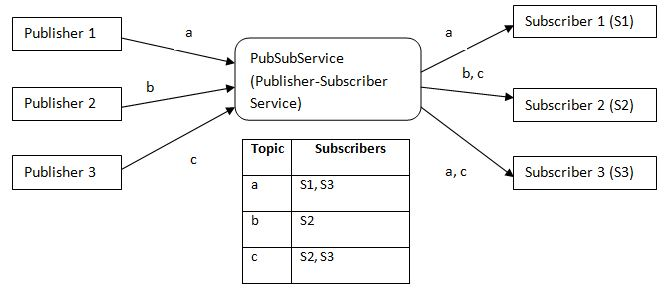
\includegraphics[scale=0.7]{Bilder/pubsub1.jpg}
	\caption[Publish-Subscribe Pattern]{Publish-Subscribe Pattern}

\end{figure}
\newline
ROS Nodes können in verschiedenen Sprachen implementiert werden, da die Kommunikation über die festen Nachrichtentypen geschieht, welche über den Roscore ausgetauscht werden. Dadurch ist es möglich Nodes in C++, Python und ebenfalls Lisp zu programmieren. Wodurch das ganze Konzept enorm flexibel gestaltet wird. Die fest definierten Nachrichtentypen verhindern, dass es an den Schnittstellen zu Problemen kommt und Nachrichten von allen Nodes einheitlich empfangen und versendet werden. \newline
Durch diese Modularität ist einfacher Komponenten und Funktionalitäten sowohl zu verwalten, als auch zu warten. Ebenfalls sind durch einheitliche Schnittstellen der Austausch von Nodes einfach und ermöglicht ein flexibles Ökosystem.

%%%%%%%%%%%%%%%%%%%%%%%%%%%%%%%%
%TODO: siehe Kommentar
% Wie wäre es, wenn wir noch sowas wie \subsection{Software Qualität} oder so machen
% und dann noch catkin build (vll auch im vergleich zu dem standard rosbuild) beschreiben
% dazu vll noch das wir alles mit startup scripten und so automatisiert haben, keine ahnung
% wäre noch ein guter filler und könnte man mit erwähnen - wäre hier in deinem Teil mit drin

%%%%%%%%%%%%%%%%%%%%%%%%%%%%%%%%
\subsection{Software Qualität}
Um die Qualität der Anwendung zu sichern wird Catkin Build anstelle des veralteten rosbuild verwendet. Bei Catkin sind Pakete der atomare Bestandteil der Anwendung.
%TODO%http://wiki.ros.org/catkin_or_rosbuild 

\section{Simulation mit Gazebo}
Da es besonders beim Flug von Quadrocoptern schnell zu Schäden kommen kann und das sowohl  in langen Ausfallzeiten, als auch zu erhöhten Materialkosten führen. Speziell beim Test von autonomen Verhalten ist der Test der Features in realer Umgebung somit mit hohem Risiko verbunden. Um dies zu vermeiden ist die Simulation von Quadrocoptern und verschiedener Umgebungen unabdingbar. Ebenfalls erleichtert eine simulierte Version der Drohne die Entwicklung, da sie nicht immer physikalisch vorhanden sein muss. Dabei ist es allerdings notwendig, insbesondere
bei Bilddaten, dass die reale Situation möglichst realitätsnah abgebildet wird, sodass
das Verhalten im realen Umfeld entsprechend ähnlich ist. Insbesondere bei der
Verarbeitung von Kameradaten ist es allerdings abzuwägen ob Ergebnisse in der Simulation
mit Resultaten in realen Umgebungen vergleichbar sind, da die simulierten
Bilddaten in der Regel eher steril sind.\newline
Durch die Integration von ROS kommt die Simulationsumgebung Gazebo als Bestandteil
mit. Anfänglich handelte es sich um ein ROS Paket, mittlerweile ist es allerdings
ein eigenständiges Ubuntupaket und benötigt de facto kein ROS.
\newline
Da die realistische Simulation einer Drohne sehr umfangreich ist wird das ROS Paket "tum simulator" verwendet. Es enthält eine Implementation der AR Drone 2.0 für den Gazebo Simulator. Es wurde von Hongrong Huang und Jürgen Sturm
 aus der Computer Vision Group von der Technischen Universität München entwickelt. Die Drohne wird komplett abstrahiert, wodurch die Simulation sich ohne Veränderung mit der realen Drohne austauschen lässt. 
 \begin{figure}[ht]
 	\centering
 	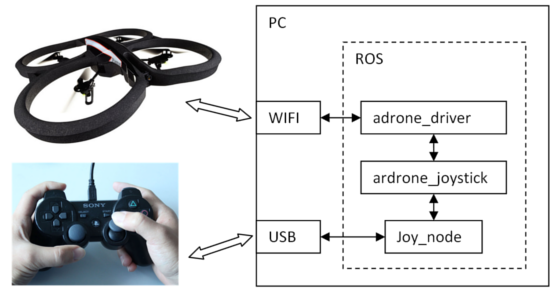
\includegraphics[scale=0.9]{Bilder/real_structure.png}
 	\caption[Programmstruktur mit dem realen Quadrocopter]{Programmstruktur mit dem realen Quadrocopter \cite{real_structure}}
 	
 \end{figure}
 Es ist auch möglich sowohl den Quadrocopter real zu steuern, als auch gleichzeitig in der Simulation. Das ermöglicht einen direkten Vergleich zwischen simulierten und realen Ergebnisse, vorausgesetzt, dass die simulierte Umgebung der echten annähernd entspricht.
  \begin{figure}[ht]
  	\centering
  	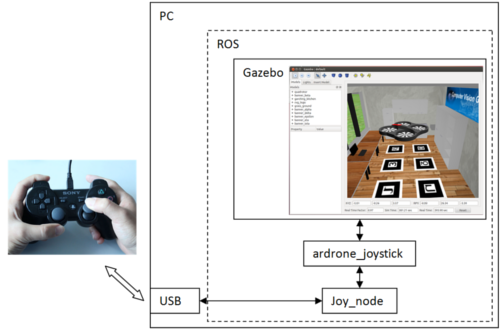
\includegraphics[scale=1.0]{Bilder/sim_structure.png}
  	\caption[Programmstruktur unter Verwendung von Gazebo]{Programmstruktur unter Verwendung von Gazebo \cite{sim_structure}}
  	
  \end{figure} %Max
Die Steuerung der Drohne, wird bei dem Package nativ über einen Playstation 3 Controller realisiert. Dessen Eingaben werden von der ROS-Node "Joy Node" verarbeitet und anschließend an die Node "ardrone joystick" weitergeleitet. Dort werden die Daten entsprechend übersetzt um entweder von Gazebo und/oder der realen Drohne verwendet werden zu können. Wenn sie an den realen Quadrocopter gesendet werden sollen, müssen sie noch entsprechend vom "ardrone driver" übersetzt werden, da lediglich Bitfolgen per WLAN versendet werden. 
\section{Fuzzylogik}
\subsection{Allgemeines}
Fuzzylogik, englisch fuzzy für unscharf oder verschwommen, ist eine Theorie die 1965 von Lotti Zadeh entwickelt wurde. Sie beschäftigt sich mit dem Modellierung von unscharfen Wissen und wird hauptsächlich für Kontrolltheorie,sowie künstliche Intelligenz verwendet. Im Gegensatz zur klassischen Logik, die als Ergebnis nur wahr oder falsch zulässt, kann man mit Fuzzylogik auch die Ausprägung einer Zugehörigkeit feststellen. Diese sogenannte \textit{Fuzziness} ermöglicht Zuordnungen wie \grqq stark\grqq \space oder \grqq ziemlich\grqq. Wesentliche Elemente sind linguistische Variablen, welche, was der Name impliziert, Wörter und Ausdrücke anstellen von Zahlen verwenden um diese unscharfen Mengen zu repräsentieren. Diesen wird eine Funktion zugeordnet um die jeweilige Ausprägung der Variable feststellen zu können.\cite{fuzzylogik} \newline
Im folgenden werden eventuell fachspezifische Terme aus der Fuzzylogik verwendet, dafür werden nachfolgende Grundbegriffe kurz erklärt:
\begin{itemize}
	\item Unscharfe Menge (fuzzy set): Mathematisches Konzept zur Darstellung vager Angaben, welches teilweise Mengenzugehörigkeit erlaubt.
	\item Unscharfe Logik (fuzzy logic): Isomorphes Konzept zur Unscharfen Menge, welches sich um den Umgang mit graduell ausgeprägten Wahrheitswerten kümmert.
	\item Unscharfe Regel (fuzzy rule): Simple Regel, deren Prädikate unscharfe Mengen enthält.
	\item Unscharfes Schließen (fuzzy reasoning): Formalisierung und Auswertung der unscharfen Regelbasen durch einen mathematischen Rahmen.
	\item Unscharfe Regelung (fuzzy control): Einbindung unscharfer regelbasierter System in technischen Anwendungen, wird auch als Fuzzy Interferenz bezeichnet \cite{fuzzybook}\cite{WissensbasierteSysteme}. 
\end{itemize}
Das verwendete Fuzzymodell besteht insgesamt aus acht linguistischen Variablen, vier Ein- und Ausgabevariablen, von welchen jede fünf Zugehörigkeitsfunktionen besitzt. Weiterhin gibt es einen Regelblock um aus den Eingaben auf die entsprechenden Ausgaben zu schließen.

\subsection{Fuzzylite}
Für die Implementation der Fuzzylogik wird die C++ Bibliothek FuzzyLite von Juan Rada-Vilela verwendet. Es handelt sich dabei um eine gratis Opensource Libary und unterstützt alle gängigen Funktionen der Fuzzylogik.\cite{fuzzylite}  
\begin{lstlisting}[caption=Beispielcode zur Erzeugung eines neuen Fuzzymodells]
void FuzzyController::init() {
	engine = new Engine;
	engine->setName("input");
	InputVariable* backward = new InputVariable;
	backward->setName("backward");
	backward->setEnabled(true);
	backward->setRange(-1.000, 1.000);
	backward->addTerm(
	new Trapezoid("strongForward", -1.000, -1.000, -0.800, -0.400));
	backward->addTerm(
	new Trapezoid("mediumForward", -0.900, -0.600, -0.400, 0.000));
	backward->addTerm(
	new Trapezoid("mediumBackward", 0.000, 0.400, 0.600, 0.900));
	backward->addTerm(
	new Trapezoid("strongBackward", 0.400, 0.800, 1.000, 1.000));
	engine->addInputVariable(backward);
}
\end{lstlisting}
Mit dem Code erzeugt man zunächst eine neue Engine und anschließend eine Eingabevariable. Dieser wird ein Wertebereich zugewiesen und Zugehörigkeitsfunktionen erstellt. Schlussendlich wird die Variable bei der Engine registriert. 
\begin{lstlisting}[caption=Code zur Erzeugung von einem Regelsystem]
RuleBlock* ruleBlock = new RuleBlock;
ruleBlock->setEnabled(true);
ruleBlock->setConjunction(new Minimum);
ruleBlock->setDisjunction(new Maximum);
ruleBlock->setImplication(new Minimum);
ruleBlock->setActivation(new General);
ruleBlock->addRule(Rule::parse(
"if backward is strongForward then backwardSpeed is strongForward",
engine));
engine->addRuleBlock(ruleBlock);
\end{lstlisting}
Mit diesem Code erzeugt man ein neues Regelsystem und fügt eine beispielhafte Regel hinzu. Ein komplettes System besteht aus wesentlich mehr Regeln, da es normalerweise komplex ist.
\begin{lstlisting}[caption=Code zur Auswertung des Regelsystems]
backward->setValue(back);
sideward->setValue(side);
up->setValue(upValue);
rotation->setValue(rotateRight);
engine->process();
\end{lstlisting}
Schließlich kann man den Eingabevariablen konkrete Werte zuweisen und das System mithilfe von unscharfen Schließen auswerten.
%Würde erwähnen dass wir es verwenden
%wollen wir das überhaupt reinnehmen? haben wir ja eigentlich gar nicht gemacht und mussten wir uns auch %null mit beschäftigen
\section{Kinect}
%Max

Um Gesten des Benutzers zur erkennen und entsprechend auszuwerten wird der visuelle Sensor Microsoft Kinect verwendet. Normalerweise wird er zur Steuerung der Videospiel Konsole Xbox360/Xbox One verwendet. Das System ist in der Lage Tiefenbilder zu erstellen, besitzt sowohl eine 1080p Farbkamera, als auch einen Infrarotsensor und mithilfe mehrere Mikrofone Sprache und Bewegung im Raum zu erkennen. Anhand der verschiedenen Kameraeingaben ist es möglich den Körper von bis zu 2 Nutzern zu erkennen und auch entsprechend zu verfolgen. Für Windows stellt Microsoft ein entsprechendes Software Development Kit (SDK) zur Verfügung um die Benutzung der Funktionalität zu vereinfachen.
%Max

\section{Punktwolken}
\label{Punktwolken}
%Christoph
Die Tiefenbilder die REMODE erstellt sind in Form von sogenannten Punktwolken, bzw. Point Clouds. Diese Punktwolken sind eine Menge von Punkten in einem Vektorraum, welche jeweils durch ihre Raumkoordinaten in einem dreidimensionalen kartesischen Koordinatensystem beschrieben sind. Somit ist jedes Element im Datensatz durch die Attribute $X$, $Y$ und $Z$ gekennzeichnet. \cite{defPC}\cite{visPC}\ \newline
Sobald ein Tiefenbild approximiert wurde, werden diese Informationen über das ROS Topic \textit{/remode/depth/pointcloud} geteilt. \newline

\begin{figure}[ht]
	\centering
	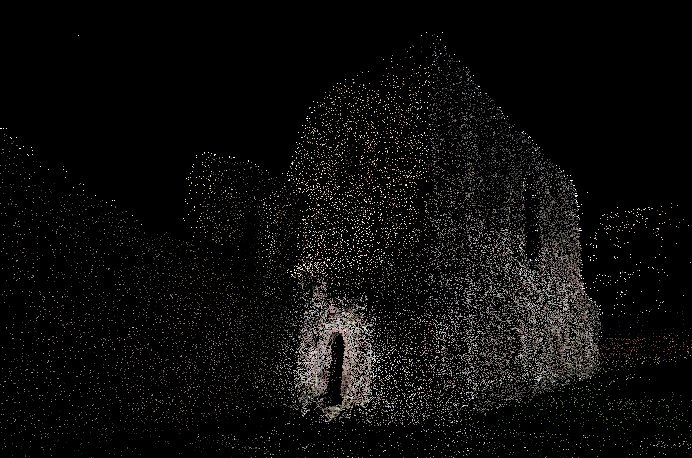
\includegraphics[scale=0.41]{Bilder/pointcloud_1.jpg}
	\label{fig:pointcloud}
	\caption{Beispiel einer visualisierten Punktwolke \cite{visPC}}
\end{figure}

Die Darstellung zeigt beispielhaft die Visualisierung einer Punktwolke. Dabei entscheidet die Helligkeit der Punkte über ihre relative Tiefe in Bezug zur Kamera. Der Vektorraum $V \in \mathbb{R}^3$ mit den entsprechenden Datenpunkten wird das ROS Topic in einem Intervall von wenigen Sekunden übertragen.\newline

\section{Point Cloud Library}
%Christoph

Die Punktwolken, wie in Abschnitt \ref{Punktwolken} beschrieben, bilden die Grundlage, um essentielle Auswertungen und Analysen für das Assistenzsystem auszuführen. Da hierfür teilweise komplexe Algorithmen und mathematische Berechnungen notwendig sind, würde die eigene Implementierung den Rahmen dieser Arbeit sprengen. \newline
Das OpenSource Projekt Point Cloud Library \emph{PCL} stellt für diesen Anwendungsfall in dessen Programmbibliothek zahlreiche Algorithmen bereit, die einfach implementiert werden können. Diese helfen bei Problemen der 2D und 3D Bildverarbeitung, sowie der Punktwolkenverarbeitung. %cite http://pointclouds.org/
Dabei werden Anwendungen in der Bildverarbeitung bereitgestellt, wie die Filterung, Segmentierung und Visualisierung von Punktwolken. \newline
Zusätzlich verfügt die PCL eine Schnittstelle zu ROS, wodurch sie sich bestens in die Projektumgebung integrieren lässt.